\section{\method}
\label{sec:toolspec}
In this section, we introduce \method, a plug-and-play SD approach for accelerating tool-calling generation. The method leverages the highly structured nature of tool calls and recurring historical patterns to construct high-quality drafts with negligible overhead. As shown in Figure~\ref{fig:toolspec}, \method integrates two complementary drafting strategies: \textit{schema-aware drafting} and \textit{retrieval-augmented speculation}, which we detail below.

\subsection{Task Formulation}
Given a user query and an input context containing system prompts and tool documentation, \method extracts tool specifications from the documentation and converts them into a structured schema. The schema defines (i) the set of schema tokens $\Sigma_{\text{schema}}$, (ii) a set of callable tools $\mathcal{C}_{\text{tools}}$ (e.g., \texttt{ForgotPassword}), and (iii) the parameter fields associated with each tool (e.g., \texttt{Status}, \texttt{Username}).

Let $\mathcal{M}$ denote the target model, $\boldsymbol{x}$ the input context, and $\boldsymbol{y} = (y_1, y_2, \ldots, y_L)$ the tool-call sequence to be generated. At decoding step $t$, following the standard SD paradigm, \method first proposes a sequence of draft tokens $\tilde{\boldsymbol{y}}_{t:t+\gamma-1} = (\tilde{y}_{t}, \tilde{y}_{t+1}, \ldots, \tilde{y}_{t+\gamma-1})$, as predictions of the subsequent decoding steps. The target model $\mathcal{M}$ then verifies these draft candidates in parallel and accepts the longest prefix that is consistent with its probability distribution. When the drafting process incurs significantly lower latency than verification, maximizing the acceptance length of $\tilde{\boldsymbol{y}}$ directly improves the effective decoding parallelism and reduces the end-to-end latency.

\begin{figure}[t]
\centering
\vspace{-0.5cm}
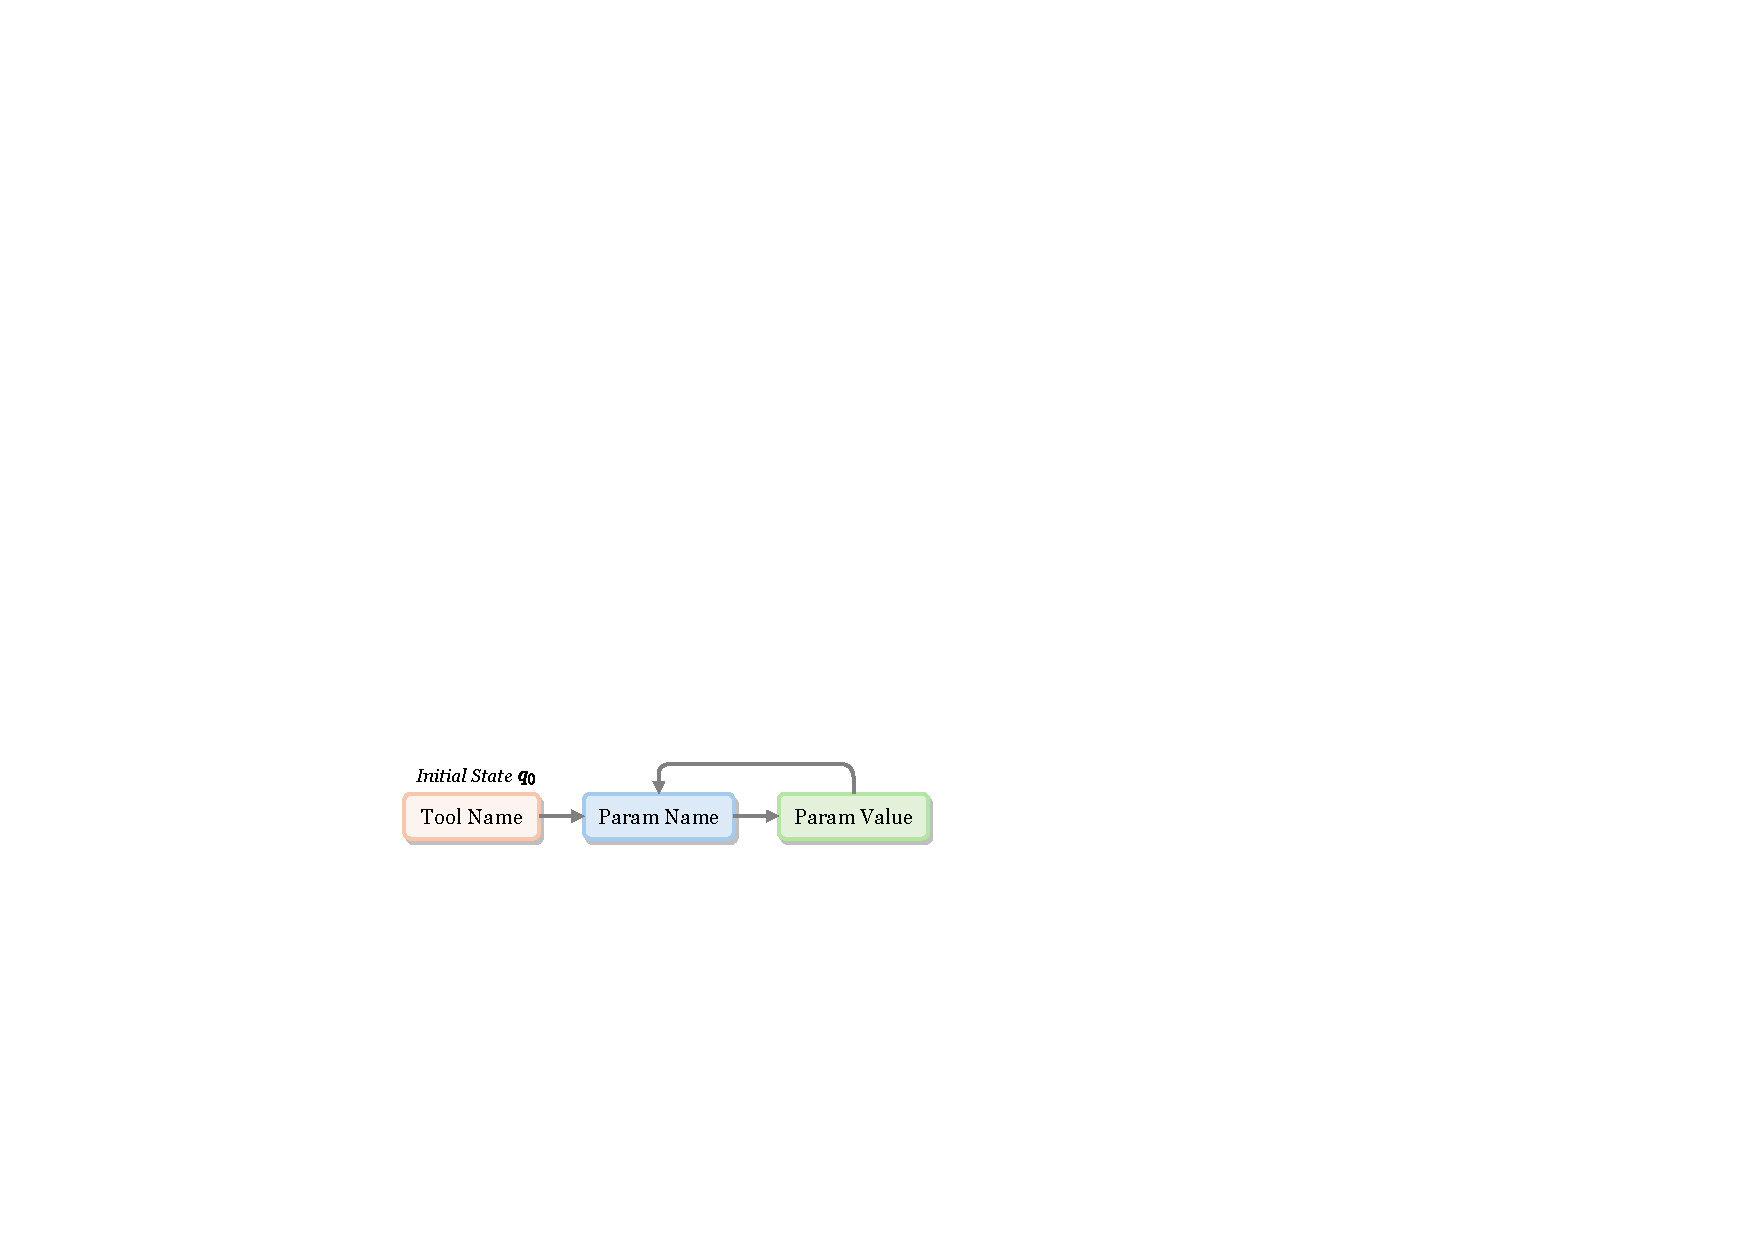
\includegraphics[width=0.95\columnwidth]{fig/transition2.pdf}
\caption{Illustration of state transitions in \method. Once tool calling is triggered by \texttt{<tool\_call>}, the FSM enters the tool-name state $q_t$, and then alternates between the parameter-name state $q_p$ and parameter-value state $q_v$ until the tool call is completed.}
\label{fig:transition}
\end{figure}

\subsection{Schema-aware Drafting}
As discussed in Section~\ref{sec:pattern_analysis}, tool invocations from advanced LLMs adhere to predefined schema formats. This structural regularity enables deterministic drafting for large portions of the output. To exploit this property, \method constructs a finite-state machine (FSM) derived from the parsed tool schema. Formally, the FSM is defined as
\begin{equation}
\mathcal{F} = (\mathcal{Q}, \Sigma_{\text{schema}}, \delta, q_0),
\end{equation}
where $\mathcal{Q}$ is the set of states, $\Sigma_{\text{schema}}$ is the schema token alphabet, $\delta: \mathcal{Q} \times \Sigma_{\text{schema}} \rightarrow \mathcal{Q}$ is the transition function, and $q_0\in \mathcal{Q}$ is the initial state.

The state space $\mathcal{Q}$ decomposes the tool-calling generation process into structural components:
\begin{itemize}
\item $q_t$: \textbf{tool-name state}, where the model selects a tool from the predefined tool set $\mathcal{C}_{\text{tools}}$.
\item $q_p$: \textbf{parameter-name state}, where the model selects one parameter field of the chosen tool.
\item $q_v$: \textbf{parameter-value state}, where the model generates the value of the selected parameter.
\item $q_o$: \textbf{``others'' state}, corresponding to general natural language generation outside tool calls.
\end{itemize}

\begin{figure*}[t]
\centering
\vspace{-1.0cm}
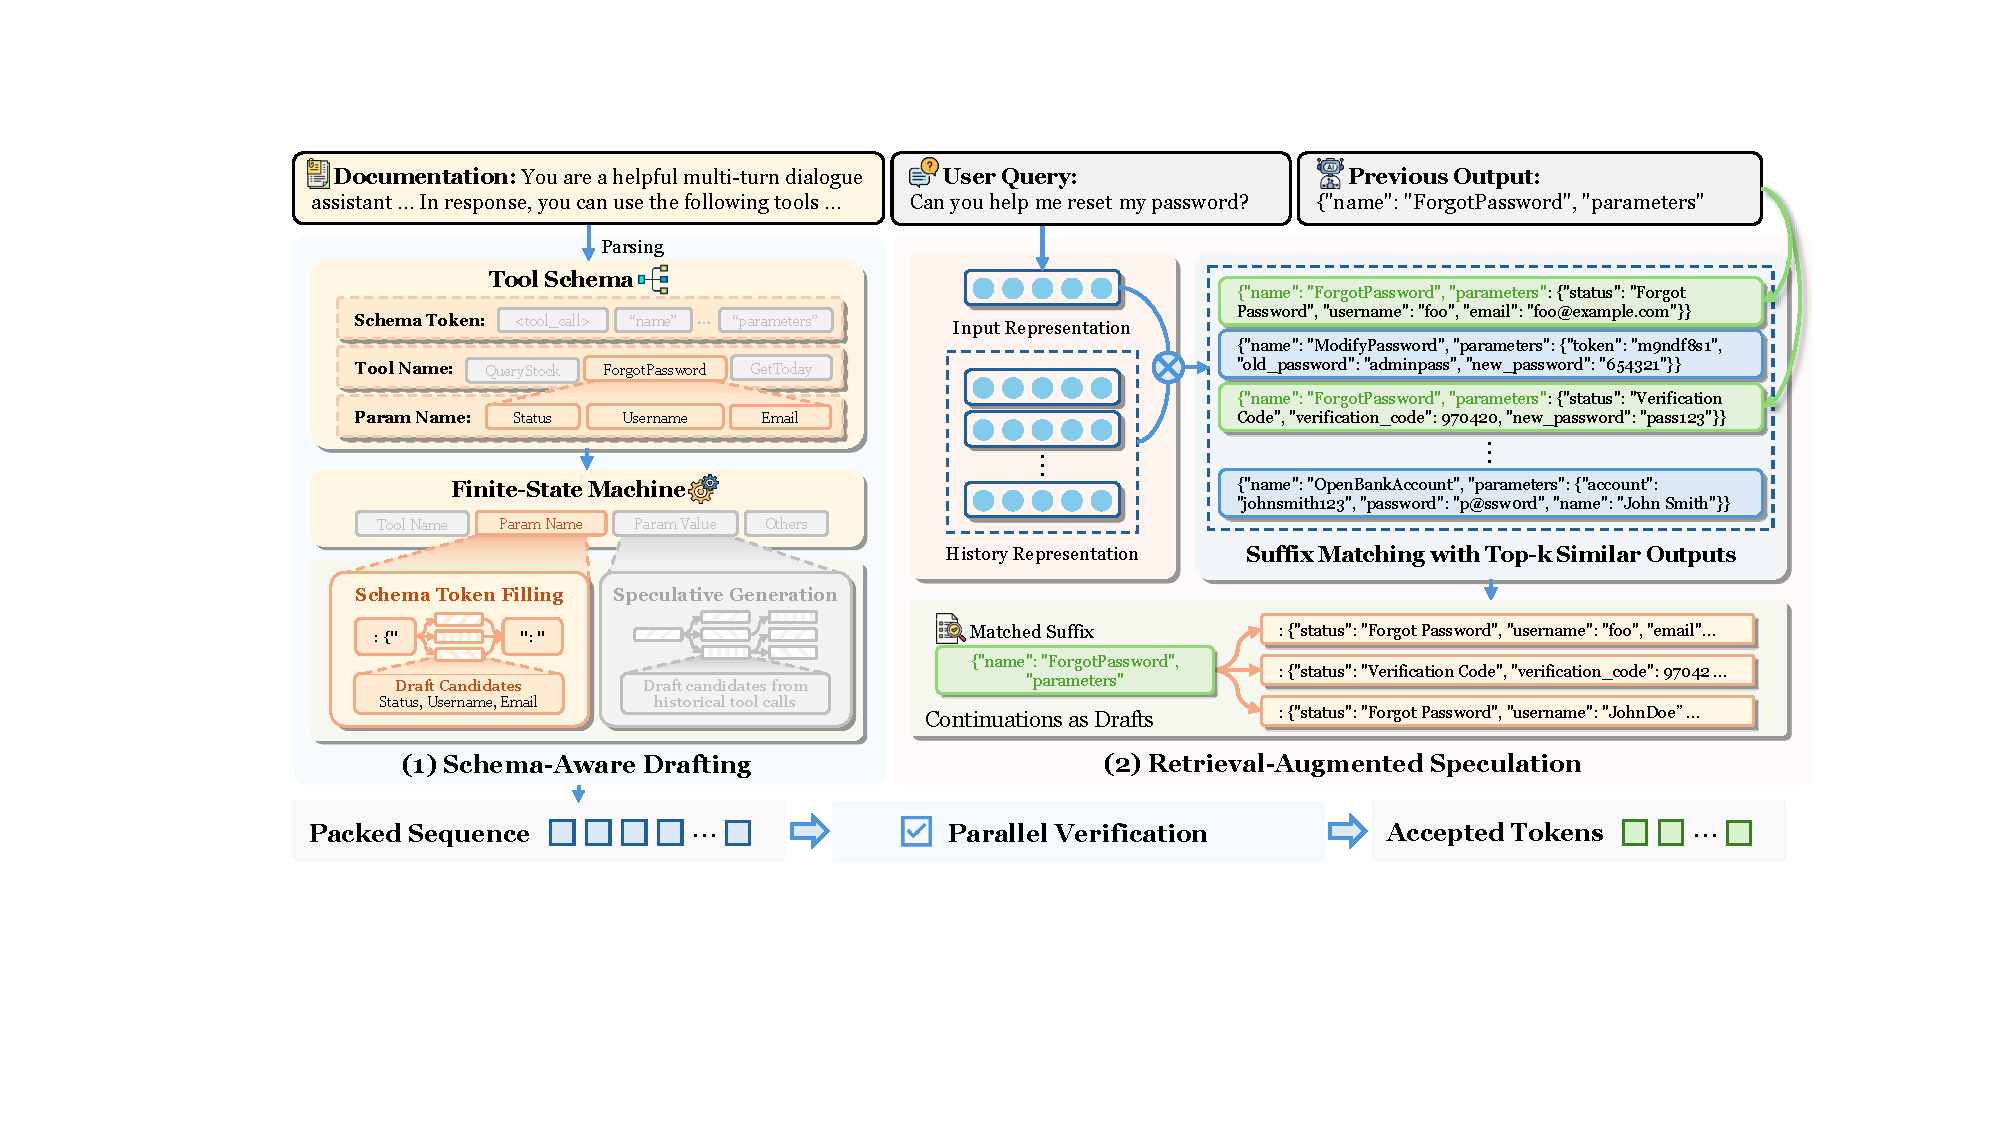
\includegraphics[width=0.95\textwidth]{fig/ToolSpec.pdf}
\caption{Illustration of tool-calling generation with \method. To accelerate structural tool calling, \method integrates two complementary drafting strategies: \textbf{(a) schema-aware drafting}, where a finite-state machine guides highly accurate drafting within the predefined tool schema; and \textbf{(b) retrieval-augmented speculation}, which reuses historical generation patterns as high-quality drafts to speed up recurrent tool calls.}
\label{fig:toolspec}
\end{figure*}

As illustrated in Figure~\ref{fig:transition}, once the special token \texttt{<tool\_call>} is generated, the FSM transitions to the tool-name state $q_t$. In this state, drafting is executed via constrained decoding to generate candidate draft sequences. We formulate the proposed draft sequence $\tilde{\boldsymbol{y}}$ as the concatenation (denoted by $\oplus$) of the necessary structural elements:
\begin{equation}\label{eq:draft}
    \tilde{\boldsymbol{y}} = \tilde{\boldsymbol{y}}_{\text{prefix}} \oplus \tilde{\boldsymbol{y}}_{\text{tool\_name}} \oplus \tilde{\boldsymbol{y}}_{\text{suffix}}
\end{equation}
where $\tilde{\boldsymbol{y}}_{\text{prefix}}$ and $\tilde{\boldsymbol{y}}_{\text{suffix}}$ denote the corresponding schema prefix and suffix associated with $q_t$, and $\tilde{\boldsymbol{y}}_{\text{tool\_name}} \in \mathcal{C}_{\text{tools}}$ represents the candidate tool names. All potential drafts are subsequently verified in parallel by the target model $\mathcal{M}$.

Upon successful verification, the FSM transitions to the parameter-name state $q_p$, where $\mathcal{M}$ verifies the candidate parameter names associated with the selected tool in parallel. The FSM then transitions to the parameter-value state $q_v$. Because parameter values are typically unconstrained, \method eschews schema constraints at this stage and instead relies on a general SD algorithm to predict these variable fields.

Then, the FSM transitions between states according to schema-specific delimiters. For example, the delimiter \mybox{delimiter}{\texttt{'',}} terminates the parameter-value state $q_v$ and returns to $q_p$ for the next parameter; while the delimiter \mybox{delimiter}{\texttt{``\}\}''}} marks completion of the tool call. Consequently, \method seamlessly alternates between deterministic schema token filling for structural states (e.g., $q_t$ and $q_p$) and speculative generation for open-ended states (e.g., $q_v$ and $q_o$).

\subsection{Retrieval-augmented Speculation}
While the schema defines the structural skeleton of a tool call and supports local drafting for constrained fields such as tool names, variable fields, particularly parameter values, depend heavily on the input context and cannot be inferred from the schema alone. Motivated by the recurring patterns in tool invocations, \method introduces a retrieval-augmented drafting strategy to accelerate tool-calling generation at the sequence level.

\begin{table*}[!t]
\centering
\vspace{-1.0cm}
\small
\setlength{\tabcolsep}{1.4mm}
\resizebox{\linewidth}{!}{
\begin{tabular}{llcccccccccc}
\toprule
\multirow{2}{*}{\textbf{Models}} & \multirow{2}{*}{\textbf{Methods}}
& \multicolumn{3}{c}{\textbf{API-Bank}}  & \multicolumn{3}{c}{\textbf{ToolAlpaca}}   & \multicolumn{3}{c}{\textbf{BFCLv2}} & \multirow{2}{*}{\begin{tabular}[c]{@{}c@{}}\textbf{Overall} \\\textbf{Speedup}\end{tabular}} \\ \cmidrule(lr){3-5} \cmidrule(lr){6-8} \cmidrule(lr){9-11} 
& &\#MAT &Tokens/s & Speedup   &\#MAT &Tokens/s & Speedup &\#MAT &Tokens/s & Speedup  \\ \midrule
\multirow{5}{*}{\begin{tabular}[c]{@{}c@{}}Qwen2.5-7B\\-Instruct\end{tabular}} & Vanilla & 1.00 & 32.76 & 1.00$\times$  & 1.00 & 32.72 & 1.00$\times$  & 1.00 & 32.73 & 1.00$\times$  & 1.00$\times$ \\
& PLD &2.37 &64.56 &1.97$\times$ &2.10 &60.75 &1.86$\times$ &2.24 &62.52 &1.91$\times$ & 1.91$\times$ \\
& TR &3.09 &78.95 &2.41$\times$ &\underline{2.87} &\underline{71.28} &\underline{2.18$\times$} &2.89 &\underline{73.64} &\underline{2.25$\times$} & \underline{2.28$\times$} \\
& SAMD &\underline{3.60} &\underline{83.96} &\underline{2.56$\times$} &2.62 &63.57 &1.94$\times$ &\underline{2.92} &70.70 &2.16$\times$ & 2.22$\times$ \\
& \blue{\method} & \blue{\bf{4.90}} &\blue{\bf{129.40}} &\blue{\bf{3.95$\times$}} & \blue{\bf{4.55}} &\blue{\bf{113.54}} &\blue{\bf{3.47$\times$}} & \blue{\bf{4.73}} &\blue{\bf{117.17}} &\blue{\bf{3.58$\times$}} &\blue{\bf{3.67$\times$}} \\\midrule
\multirow{6}{*}{\begin{tabular}[c]{@{}c@{}}Qwen2.5-14B\\-Instruct\end{tabular}} & Vanilla & 1.00 & 19.50 & 1.00$\times$  & 1.00 & 19.02 & 1.00$\times$ & 1.00 & 19.31 & 1.00$\times$  &1.00$\times$  \\
& PLD &1.98 &35.30 &1.81$\times$ &2.00 &34.85 &1.83$\times$ &2.02 &35.34 &1.83$\times$ &1.82$\times$\\
& TR &3.01 &\underline{46.94} &\underline{2.41$\times$} &2.85 &\underline{41.97} &\underline{2.21$\times$} &2.99 &\underline{46.34} &\underline{2.40$\times$} &\underline{2.34$\times$}\\
& SAMD &2.93 &45.86 &2.35$\times$ &2.62 &38.48 &2.02$\times$ &2.78 &42.29 &2.19$\times$ &2.19$\times$\\
& \gray{Eagle-2$^*$} & \gray{\underline{3.87}} & \gray{46.80}  & \gray{2.40$\times$} & \gray{\underline{3.58}} & \gray{36.24} & \gray{1.91$\times$} &\gray{\underline{3.67}} & \gray{39.39} & \gray{2.04$\times$} &\gray{2.12$\times$} \\
& \blue{\method} & \blue{\bf{4.43}} &\blue{\bf{75.27}} &\blue{\bf{3.86$\times$}} & \blue{\bf{4.02}} &\blue{\bf{60.86}} &\blue{\bf{3.20$\times$}} & \blue{\bf{4.15}} &\blue{\bf{65.07}} &\blue{\bf{3.37$\times$}} &\blue{\bf{3.48$\times$}}\\\midrule
\multirow{6}{*}{\begin{tabular}[c]{@{}c@{}}LLaMA-3.1-8B\\-Instruct\end{tabular}} & Vanilla & 1.00 & 28.21 & 1.00$\times$ & 1.00 & 27.69 & 1.00$\times$ & 1.00 & 27.83 & 1.00$\times$ &1.00$\times$ \\
& PLD & 2.35 & 60.72  & 2.15$\times$ & 2.27 & 58.28 & 2.10$\times$ &2.30 & 58.72 &2.11$\times$ &2.12$\times$ \\
& TR & \underline{3.34} & \underline{71.10}  & \underline{2.52$\times$} & \underline{3.32} & \underline{67.69} & \underline{2.44$\times$} &\underline{3.29} &\underline{66.79} &\underline{2.40$\times$} &\underline{2.45$\times$} \\
& SAMD  & 3.20 & 69.68 & 2.47$\times$ & 3.12 & 65.82 & 2.38$\times$ &3.14 &66.24 & 2.38$\times$ &2.41$\times$ \\
& \gray{Eagle-3$^*$} & \gray{\underline{3.34}} & \gray{47.24}  & \gray{1.67$\times$} & \gray{2.93} & \gray{40.37} & \gray{1.46$\times$} &\gray{3.17} & \gray{42.86} & \gray{1.54$\times$} &\gray{1.56$\times$} \\
& \blue{\method} &\blue{\bf{5.80}} &\blue{\bf{125.59}} &\blue{\bf{4.45$\times$}} &\blue{\bf{5.26}} &\blue{\bf{112.26}} &\blue{\bf{4.05$\times$}} &\blue{\bf{5.31}} &\blue{\bf{113.55}} &\blue{\bf{4.08$\times$}} &\blue{\bf{4.19$\times$}} \\\midrule
\multirow{5}{*}{\begin{tabular}[c]{@{}c@{}}LLaMA-3.2-3B\\-Instruct\end{tabular}} & Vanilla & 1.00 & 32.60 & 1.00$\times$  & 1.00 & 33.20 & 1.00$\times$  & 1.00 & 32.91 & 1.00$\times$  & 1.00$\times$  \\
& PLD &2.19 &69.81 &2.14$\times$ &2.06 &61.41 &1.85$\times$ &2.11 &64.83 &1.97$\times$ &1.99$\times$\\
& TR &\underline{3.11} &\underline{75.50} &\underline{2.32$\times$} &\underline{3.03} &\underline{73.45} &\underline{2.31$\times$} &\underline{3.06} &\underline{76.35} &\underline{2.32$\times$} &\underline{2.32$\times$}\\
& SAMD &2.99 &72.79 &2.18$\times$ &2.68 &71.84 &2.16$\times$ &2.75 &71.09 &2.16$\times$ &2.17$\times$\\
& \blue{\method} & \blue{\bf{5.20}} &\blue{\bf{133.30}} &\blue{\bf{4.09$\times$}} & \blue{\bf{4.52}} &\blue{\bf{112.22}} &\blue{\bf{3.38$\times$}} & \blue{\bf{4.78}} &\blue{\bf{115.84}} &\blue{\bf{3.52$\times$}} &\blue{\bf{3.66$\times$}}\\
\bottomrule
\end{tabular}}
\caption{Comparison of inference efficiency between \method and prior plug-and-play methods. We report the mean number of accepted tokens (\#MAT), average decoding speed (tokens/s), and wall-clock speedup relative to vanilla autoregressive decoding. The best results are shown in \textbf{boldface}, and the second-best results are \underline{underlined}. \gray{$^*$The Eagle series, a training-required SD method, is included for reference only.}}
\label{tab:main-exp}
\end{table*}

We maintain a datastore $\mathcal{H}=\{(\boldsymbol{h}_j, \boldsymbol{y}_j)\}_{j=1}^{|\mathcal{H}|}$ consisting of prior successful tool calls, where $\boldsymbol{h}_j \in \mathbb{R}^d$ denotes the hidden representation of the input question $\boldsymbol{x}_j$ at its final token, $d$ is the hidden dimension, and $\boldsymbol{y}_j$ is the corresponding tool-call output. Given a query $\boldsymbol{x}_i$, we retrieve the top-$k$ most similar historical tool calls:

\begin{equation}
    \mathcal{I}_k = \operatorname{Top-K}_{j \in \{1 \ldots |\mathcal{H}|\}} \text{sim}(\boldsymbol{h}_i, \boldsymbol{h}_j)
\end{equation}
where $\text{sim}(\cdot)$ denotes cosine similarity and $\mathcal{I}_k$ the indices of the retrieved entries. Given the partially generated output $\boldsymbol{y}_{<t}$, we align it with each retrieved tool call $\boldsymbol{y}^{\prime}$ by matching the suffix:
\begin{equation}
\boldsymbol{y}_{t-L:t-1}=\boldsymbol{y}^{\prime}_{m-L:m-1}
\end{equation}
where $L$ denotes the suffix length and $m$ indicates the corresponding match position in $\boldsymbol{y}^{\prime}$. When a suffix match is found, \method extracts the next $n$ tokens $\boldsymbol{y}^{\prime}_{m:m+n-1}$, using these continuations as drafts. As shown in Figure~\ref{fig:toolspec}, if the current suffix matches a historical invocation containing \mybox{delimiter}{...``parameters''}, the subsequent tokens (e.g., \mybox{delimiter}{:\{``status'': ``Forgot Password''...}) are proposed as draft candidates. Intuitively, once the tool name and key–value pairs are aligned, the remaining structure of the tool call often follows recurring patterns, making $\boldsymbol{y}'_{m:m+n-1}$ high-quality drafts for subsequent value spans.

